\section{\textbf{Applications with AME}}

We apply AME to three recent IR studies: \citet{reiter:stam:2003, weeks:2012, gibler:2017}. Each of these studies use relational data of state interactions and propose both dyadic, monadic, and structural explanations for behavior of actors in the system. We choose to demonstrate the capabilities of AME with reference to existing studies in order to highlight several features of our network based approach. First, we show that simply by using the AME framework scholars can better model the data generating process behind their events of interest. Second, the results of AME estimation are interpretable alongside results using standard approaches, but, as shown in the simulation section, have the additional benefit of being able to take into account dependencies that may otherwise complicate inference. Third, through using this approach, we can also quantify the degree to which first, second, and third order dependencies are present in events of interest.

We obtained the data for these studies from their replication archives.\footnote{Without exception the data was easy to retreive thanks to the authors' transparency and an increasing norm in the social sciences of open data sharing.} The studies below were selected based on how recently they were published and whether they had more then 100 citations.\footnote{Note that we chose papers with at least 100 citations as an indicator of influence within the discipline. Of course, by the criteria of influence many other papers could have been considered for the replication.} Each of these pieces, published in prominent journals well-known in their respective literatures, posited a theory in which interdependencies are consequential. Reflecting the dominant approach in the literature, the studies tested their hypothesis by employing some form of a general linearized model. Table~\ref{tab:modelDesign} provides descriptive information for the studies that we replicated.
% \footnote{It is important to note that the AME framework is not well suited for studies where the focus may be on studying onsets as in these type of studies dyad-years representing conflict continuations are removed from the sample. In studies with this type of focus, network models in general are of limited utility since any interdependencies underlying how events may spread from one actor to another are explicitly masked from the estimation process due to the removal of observations.} ........... gibler uses a study onsets. in some ways this is problematic in other it is not, i'm (sm) suggesting that we ignore for now.

\begin{table}
\caption{Descriptive information about the replicated studies. }
	\begin{tabular}{lccccc}
		& Model &  Date Range & N. Actors  & Dyads Type & Clustering $\sigma_{\hat{\beta}}$ \\ \toprule
		Reiter \& Stam (2003) & Logit &1945--1995 &  193 & Directed & Robust \\	
		Weeks (2012) & Logit & 1946--1999 & 197 & Directed & Robust \\
		Gibler (2017) & Logit & 1816--2008 & 193 & Undirected & Robust \\ \bottomrule
	\end{tabular}
	\label{tab:modelDesign}
\end{table}

From each of the studies listed above we replicated the authors' key model using their original estimation procedure, a generalized linear model.\footnote{Replicating the key models from each study was straightforward to do because of the authors' neatly assembled replication scripts.} Next, utilizing the same covariate specifications, we estimated the models with the AME framework.\footnote{In estimating AME, we show results when setting $K=2$. Results with alternative values of $K$ are similar.} For \citet{reiter:stam:2003, weeks:2012}, we utilized a version of AME that accounts for the directed nature of the data and for \citet{gibler:2017} we used an undirected version. In the directed formulation, separate random effects are used for senders and receivers in both the additive and multiplicative portions of the model. 

A key claim that we have made is that by accounting for dependencies inherent in relational data we can better capture the data generating process behind events of interest. To assess whether or not the AME approach successfully does this, we turn to an out-of-sample cross validation strategy. An out-of-sample approach here is essential as relying on in-sample procedures would enable models with more parameters, such as AME, to simply overfit the data. The cross validation procedure works as follows, for each study, we randomly divide the data into $k=30$ sets, letting $s_{ij,t}$ be the set to which pair $ij,t$ is assigned. Then for each $s \in \{1,\ldots,k\}$, we:

\begin{enumerate}
	\item estimate model parameters with $\{y_{ij,t}: s_{ij,t} \neq s\}$, the data not in set $s$,
	\item and predict $\{\hat{y}_{ij,t}: s_{ij,t} = s\}$ from these estimated parameters. 
\end{enumerate}

The result of this procedure is a set of sociomatrices $\bm \hat Y$, in which each entry $\hat y_{ij,t}$ is a predicted value obtained from using a subset of the data that does not include $y_{ij,t}$. For each study we next conducted a series of analyses to discern whether or not the AME model provides any benefit. These analyses are summarized in Figure~\ref{fig:perf}. The left-most plot in each of the panels evaluates performance using Receiver Operating Characteristic (ROC) curves. Models that have a better fit according to this metric will follow the left-hand and then top borders of the ROC space. In addition, to ROC curves we also use separation plots, these visualize each of the observations in the dataset according to their predicted probability. Observations in which there is an actual link are colored in by the modeling approach. Models with a better fit should have the majority of colored links towards the right end of the plot. The right-most plot in each of the panels evaluates performance using precision-recall (PR) curves. PR curves are useful in situations where correctly predicting events is more interesting than simply predicting non-events \citep{davis:goadrich:2006}. This is especially relevant in the context of our applications here, as they each are trying to model conflict in a dyadic setting, which is an infrequent occurrence. 

For each of the replications, we find that the AME approach substantially outperforms the original models in terms of out-of-sample predictive performance. This indicates that switching to the AME framework---even when using the same covariate specification as the original studies---enables scholars to better represent the data generating process of their events of interest. The fact that this analysis is done in an out-of-sample context ensures that the AME framework is not simply overfitting with more parameters, rather the additive and multiplicative effects we include are capturing underlying structure previously missed by the exogenous covariates in the models.

\begin{figure}
	\centering   
	\begin{tabular}{cc}
		\multicolumn{2}{l}{\textbf{\tiny{Reiter \& Stam (2003)}}} \\
		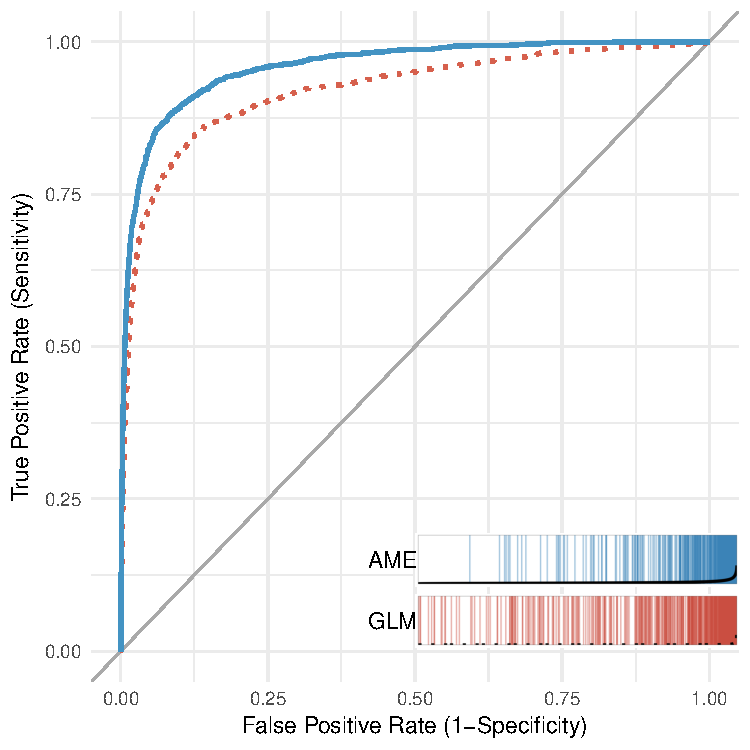
\includegraphics[width=.4\textwidth]{graphics/reiter_stam_roc_outSample.pdf} & 
		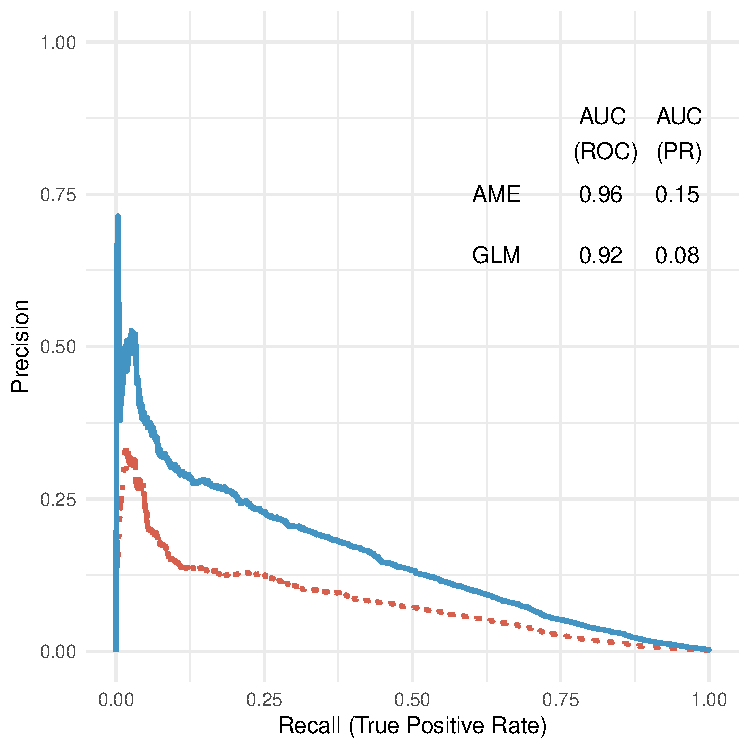
\includegraphics[width=.4\textwidth]{graphics/reiter_stam_pr_outSample.pdf} \\
		\multicolumn{2}{l}{\textbf{\tiny{Weeks (2012)}}} \\
		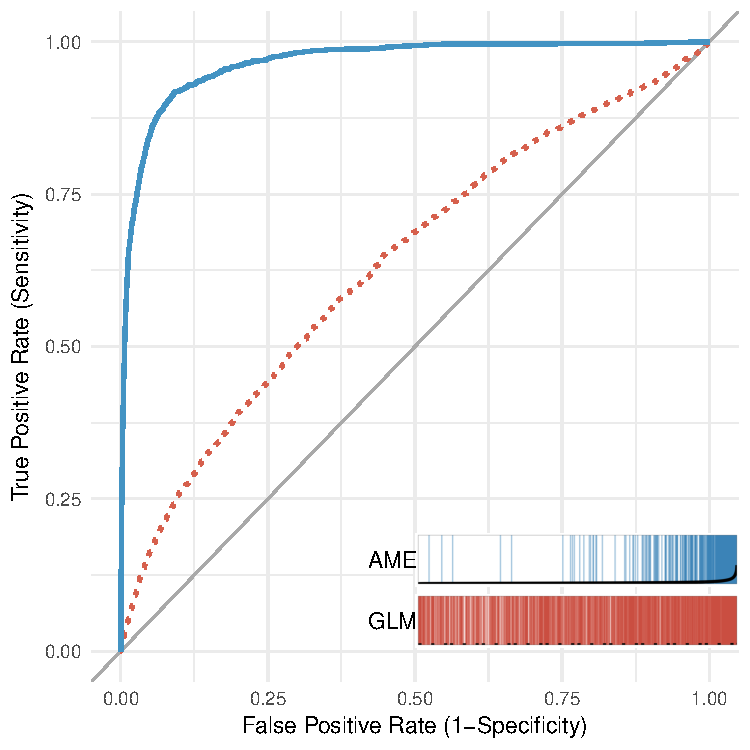
\includegraphics[width=.4\textwidth]{graphics/weeks_roc_outSample.pdf} & 
		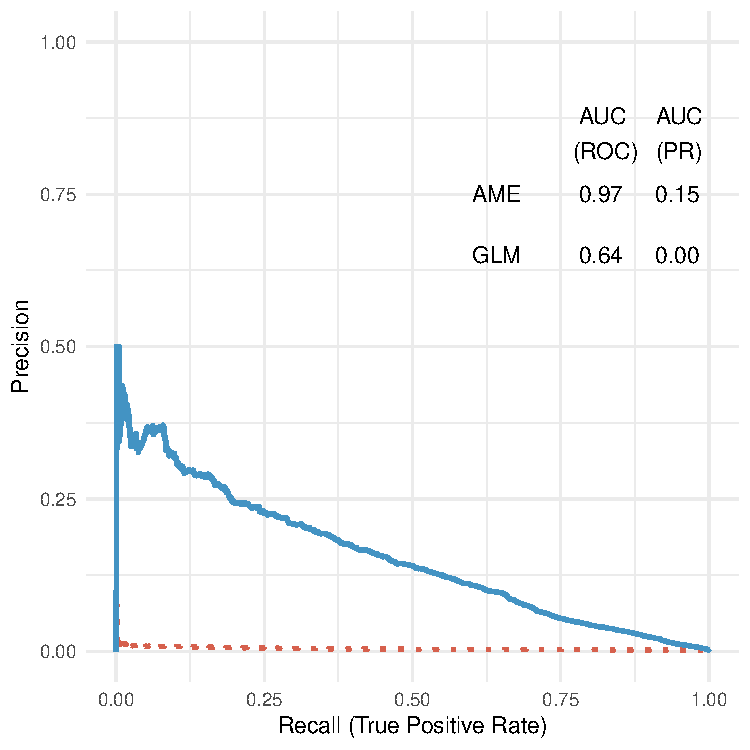
\includegraphics[width=.4\textwidth]{graphics/weeks_pr_outSample.pdf} \\
		\multicolumn{2}{l}{\textbf{\tiny{Gibler (2017)}}} \\
		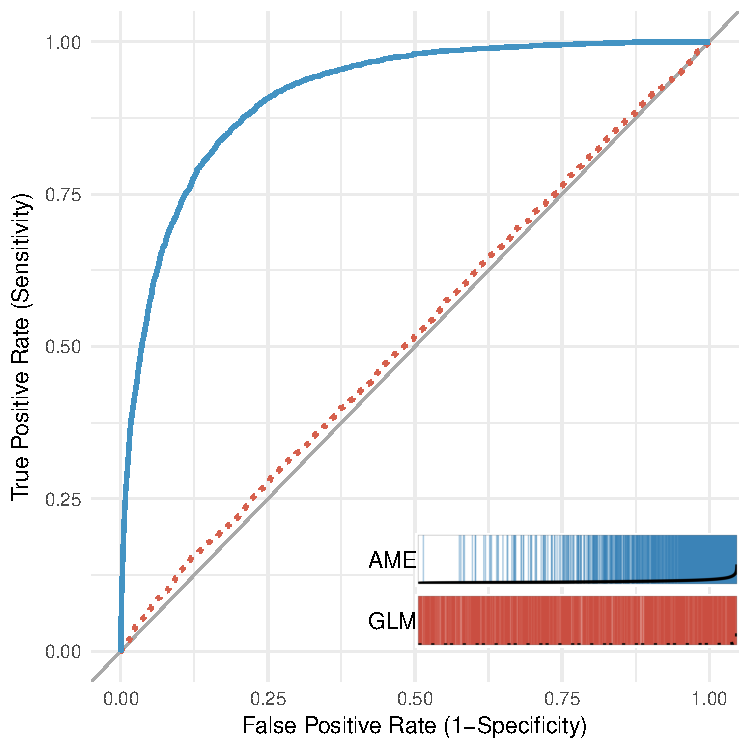
\includegraphics[width=.4\textwidth]{graphics/gibler_roc_outSample.pdf} & 
		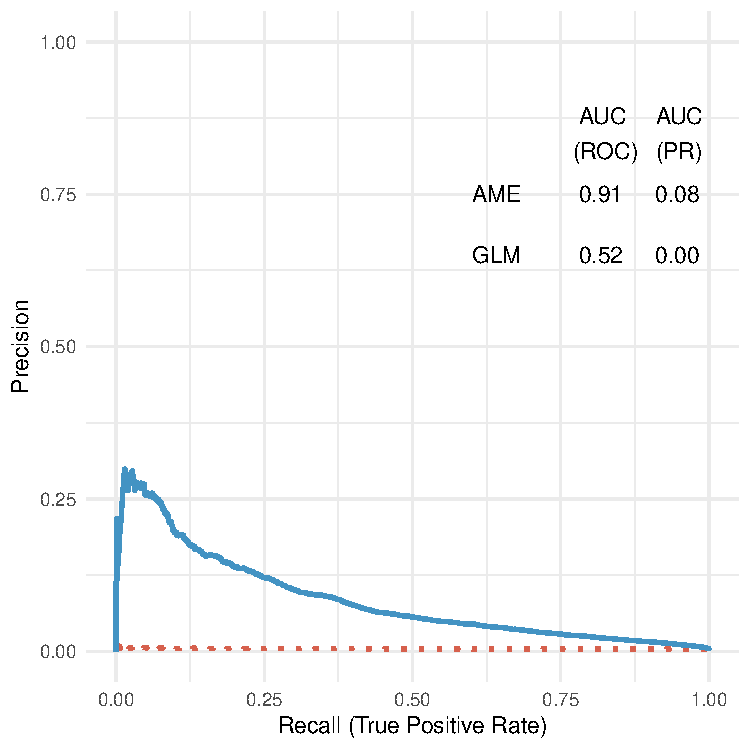
\includegraphics[width=.4\textwidth]{graphics/gibler_pr_outSample.pdf} \\
	\end{tabular}
	\caption{Assessments of out-of-sample predictive performance using ROC curves, PR curves, and separation plots.}
	\label{fig:perf}	
\end{figure}

Ignoring this underlying structure has implications when trying to draw inferences about the effects of covariates.\footnote{As shown in the simulation section, inference in a dyadic setting can become complicated when there are unobserved dependencies.} The fact that there is such a divergence in the performance of AME versus the original estimation procedures highlights that there are unobserved sources of bias in each of these studies. We hone in on the main finding of the studies to draw into focus the potential consequences for ignoring these sources of bias and the inferential benefits of the AME estimation procedure.  In Table~\ref{tab:modelFindingSumm}, we present the overall results; the term \textit{Unconfirmed} indicates only that the sign and/or significance of the crucial finding in the original study is not found to hold in the AME estimation.\footnote{Full tabular results for each of the original and reestimated models are presented in the Appendix.}

\begin{table}[ht]
\centering
\caption{Here we provide a brief summary of the key variable in each of the replications and a note about whether or not the highlighted finding remains when using our network-based approach.}
	\begin{tabular}{l p{6cm} l} \toprule
		\multirow{2}{*}{Study} & \multirow{2}{*}{Central Finding} &  Confirmed after \\
		& &  accounting for dependencies? \\ \toprule
		Reiter \& Stam (2003) & Personalist Regimes Attack Democracies, Not Vice Versa & {Confirmed} \\ \midrule
		Weeks (2012) & Bosses, Juntas, and Strongmen are more Aggressive, Machines are Not & {Unconfirmed} \\\midrule
		Gibler (2017) & Power Parity at Time of Entry to International System Increases Conflict & {Unconfirmed}\\ \bottomrule
	\end{tabular}
	\label{tab:modelFindingSumm}
\end{table}

An important takeaway here is that many scholars are forced to make knowledge claims based on the statistical significance of a small set of covariates, or the differences between these covariates. These differences may change dramatically when interdependencies are taken into account directly. This outcome follows from AME's ability to better account for the dependencies discussed in the previous section, whereas GLM approaches explicitly assume observational independence conditional on the specified covariates. As this is a widely-known limitation of GLM approaches, scholars often attempt to account for clustering of observations by including additional variables and adjusting the standard errors of the resulting estimates. At best, this method introduces noise and imprecision into results, and at worst can produce misleading outcomes. 

Next we discuss each of the replications in more detail and highlight the substantive insights that can be drawn from the AME framework.

\subsection{Reiter \& Stam (2003)}

\citet{reiter:stam:2003} examine the relationship between democracy, dictatorship and the initiation of militarized disputes. Their work contests prior scholarship that had claimed interstate dyads containing democracies and personalist dictatorships were particularly prone to conflict because of aggression on the part of the democratic state \citep{peceny:etal:2002}. Using a directed dyadic dataset of almost a million observations, they find evidence against this hypothesis: dictators are in fact more likely to challenge democracies, but not the other way around. In addition, military regimes and single-party regimes are more prone to initiate disputes with democracies, but the opposite is not true.\footnote{Independent variables focus on various encodings of regime types, contiguity, alliance, and capability measures. For a full tabular display of the results see the Appendix.} As is prevalent in this literature, Reiter \& Stam employ a logistic regression that includes an indicator of the time since the last dispute as well as three cubic splines. Based on their statistical analysis, they conclude that institutional constraints affect the propensity of democratic and non-democratic leaders to engage in military conflict. 

The key variables in their original model were indicator for whether or not the sender in the directed dyad is a personalist regime and the target a democratic (``Pers/Democ directed dyad"), and whether the sender was a democratic regime and the target personalist (``Democ/Personalist directed dyad''). They had found that the Pers/Democ Directed Dyad indicator was positive, while the Democ/Personalist directed dyad is too imprecisely measured to indicate a direction. In our re-estimation using the AME framework, we confirm these results, indicating that dictators are more likely to initiate or be in conflict with democratic regimes but not vice versa. 

Though we are able to confirm their results it is not the case that employing the AME model does not still come with benefits. As already shown in Figure~\ref{fig:perf}, our approach performs notably better in reflecting the data generating process. The reason for this is that there is still underlying structure within this conflict system that the Reiter \& Stam model does not fully capture. To highlight this we visualize the estimated sender random effects ($a_{i}$) from the SRRM portion of the AME framework in Figure~\ref{fig:reiter_stam_aEff}. 

\begin{figure}[ht]
	\begin{tabular}{cc}
	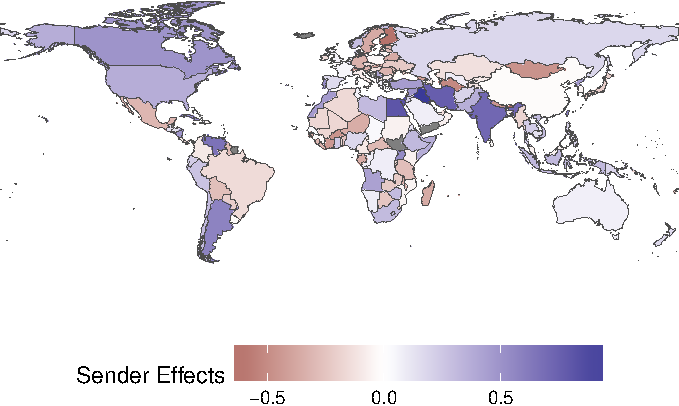
\includegraphics[width=.7\textwidth]{graphics/reiter_stam_aEff_map.pdf} &
	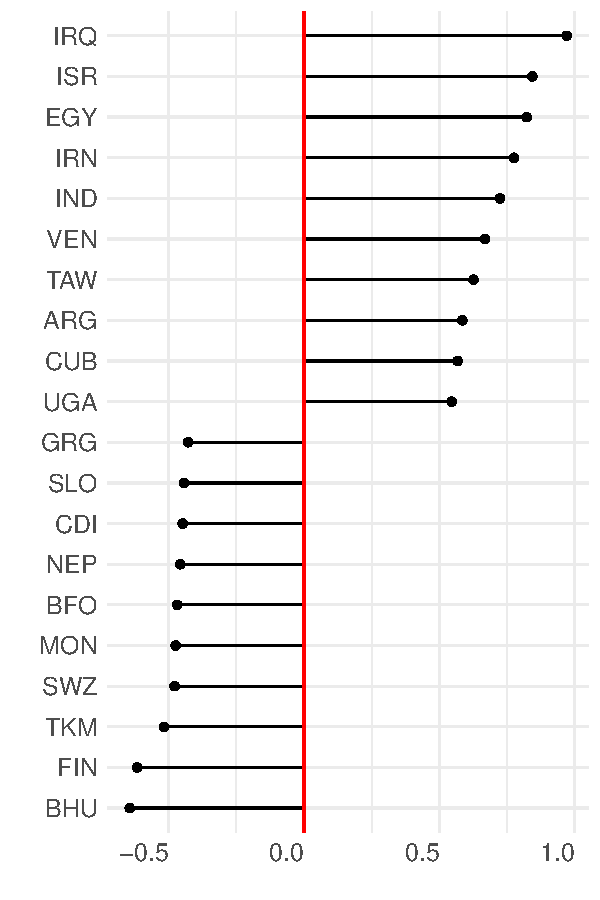
\includegraphics[width=.3\textwidth]{graphics/reiter_stam_aEff_line.pdf} \\
	\end{tabular}
	\caption{Estimates of sender random effects ($a_{i}$) from AME for the Reiter \& Stam (2003) model. Positive values indicate that the particular country is more likely to be involved in conflict than predicted by the covariates in the model, and negative values indicate that the country is less likely to be involved in conflict. Left-panel shows $a_{i}$ estimates for all countries and right-panel highlights the top ten countries in terms of positive and values of $a_{i}$.}
	\label{fig:reiter_stam_aEff}
\end{figure}
\FloatBarrier

The visualization of the sender random effects highlights that the behavior of a number of countries does not fully accord with predictions from the covariates specified by Reiter \& Stam. Specifically, we can see that countries such as Iraq, Israel, Egypt, and Iran are more likely to be involved in initiating or continuing conflict with other countries than what the covariates specified in the model would predict. Further other countries such as Bhutan, Finland, and Turkmenistan are less likely to engage in conflict than what the fixed effects in the model would predict. None of these findings change the key conclusion from Reiter \& Stam's work, but by using the AME framework we are able to better understand the limitations of their model.

\subsection{Weeks (2012)}

\citet{weeks:2012} examines the influence of domestic institutions on the initiation of military conflicts by autocratic leaders. She argues that in some circumstances autocrats are held accountable for their foreign policy decisions, and that this is dependent on the audiences of autocrats. When the autocratic regime is nonmilitary, domestic audiences do not favor military actions, but in military autocracies this is not the case. Further she argues that in personalistic regimes without a military or civilian domestic audience, the leaders tend to be more likely to employ military force in their foreign policy. To study this question, Weeks employs a directed dyad design of conflict similar to that used by Reiter \& Stam.

The major innovation in her study resides in the nuanced way in which she conceptualizes and codes regimes into four types: a) Machine, b) Junta, c) Boss, and d) Strongmen.\footnote{Weeks also includes a variety of control variables focusing on capabilities for both sides of the dyad, alliances, geography, trade dependence, regime instability, and the regime type of ``side B.'' For a full tabular display of the results see the Appendix.} She uses a logistic regression, but follows \citet{beck:etal:1998} and includes splines to capture temporal covariation in the dependent variable along with fixed, unit effects. The key finding of this work is that a) juntas, boss type, and strongmen type regimes are more likely to initiate conflict than machine-type regimes and that b) machine-type regimes are no more belligerent than democracies.\footnote{These insights are mainly emphasized in the paper by the parameter estimates depicted in Tables 1 and 2 (pages 339--340) from the paper.} In the empirical analysis, Weeks finds that machines are less prone to initiate conflict than the reference category, whereas Juntas, Bosses, and Strong-men are more conflict-prone. When analyzing the results using AME, however, we find that the parameters on each of her autocratic regime type variables are too imprecisely measured to draw any inferences. The implication being that none of the findings from her original analysis are confirmed when accounting for dependencies. 

There is also a striking difference in terms of the ability of Weeks' original model and our estimation using AME in terms of capturing the data generating process. Specifically, The area under the ROC curve for AME and GLM models are 0.97 and 0.64, respectively, which is a dramatic difference given that both models are employing the same fixed effects. As with Reiter \& Stam, the divergence is a result of the GLM framework not being able to account for underlying structure in the event of interest. To uncover some of this structure, we illustrate another beneficial aspect of the AME framework, which is the multiplicative random effects estimated through the LFM portion of the model -- $\mathbf{u}_{i}^{\top} \mathbf{D} \mathbf{v}_{j}$. These random effects account for higher order dependencies in relational data that manifest as a result of the presence of homophily and stochastic equivalence in dyadic data. 

\begin{figure}[!h]
	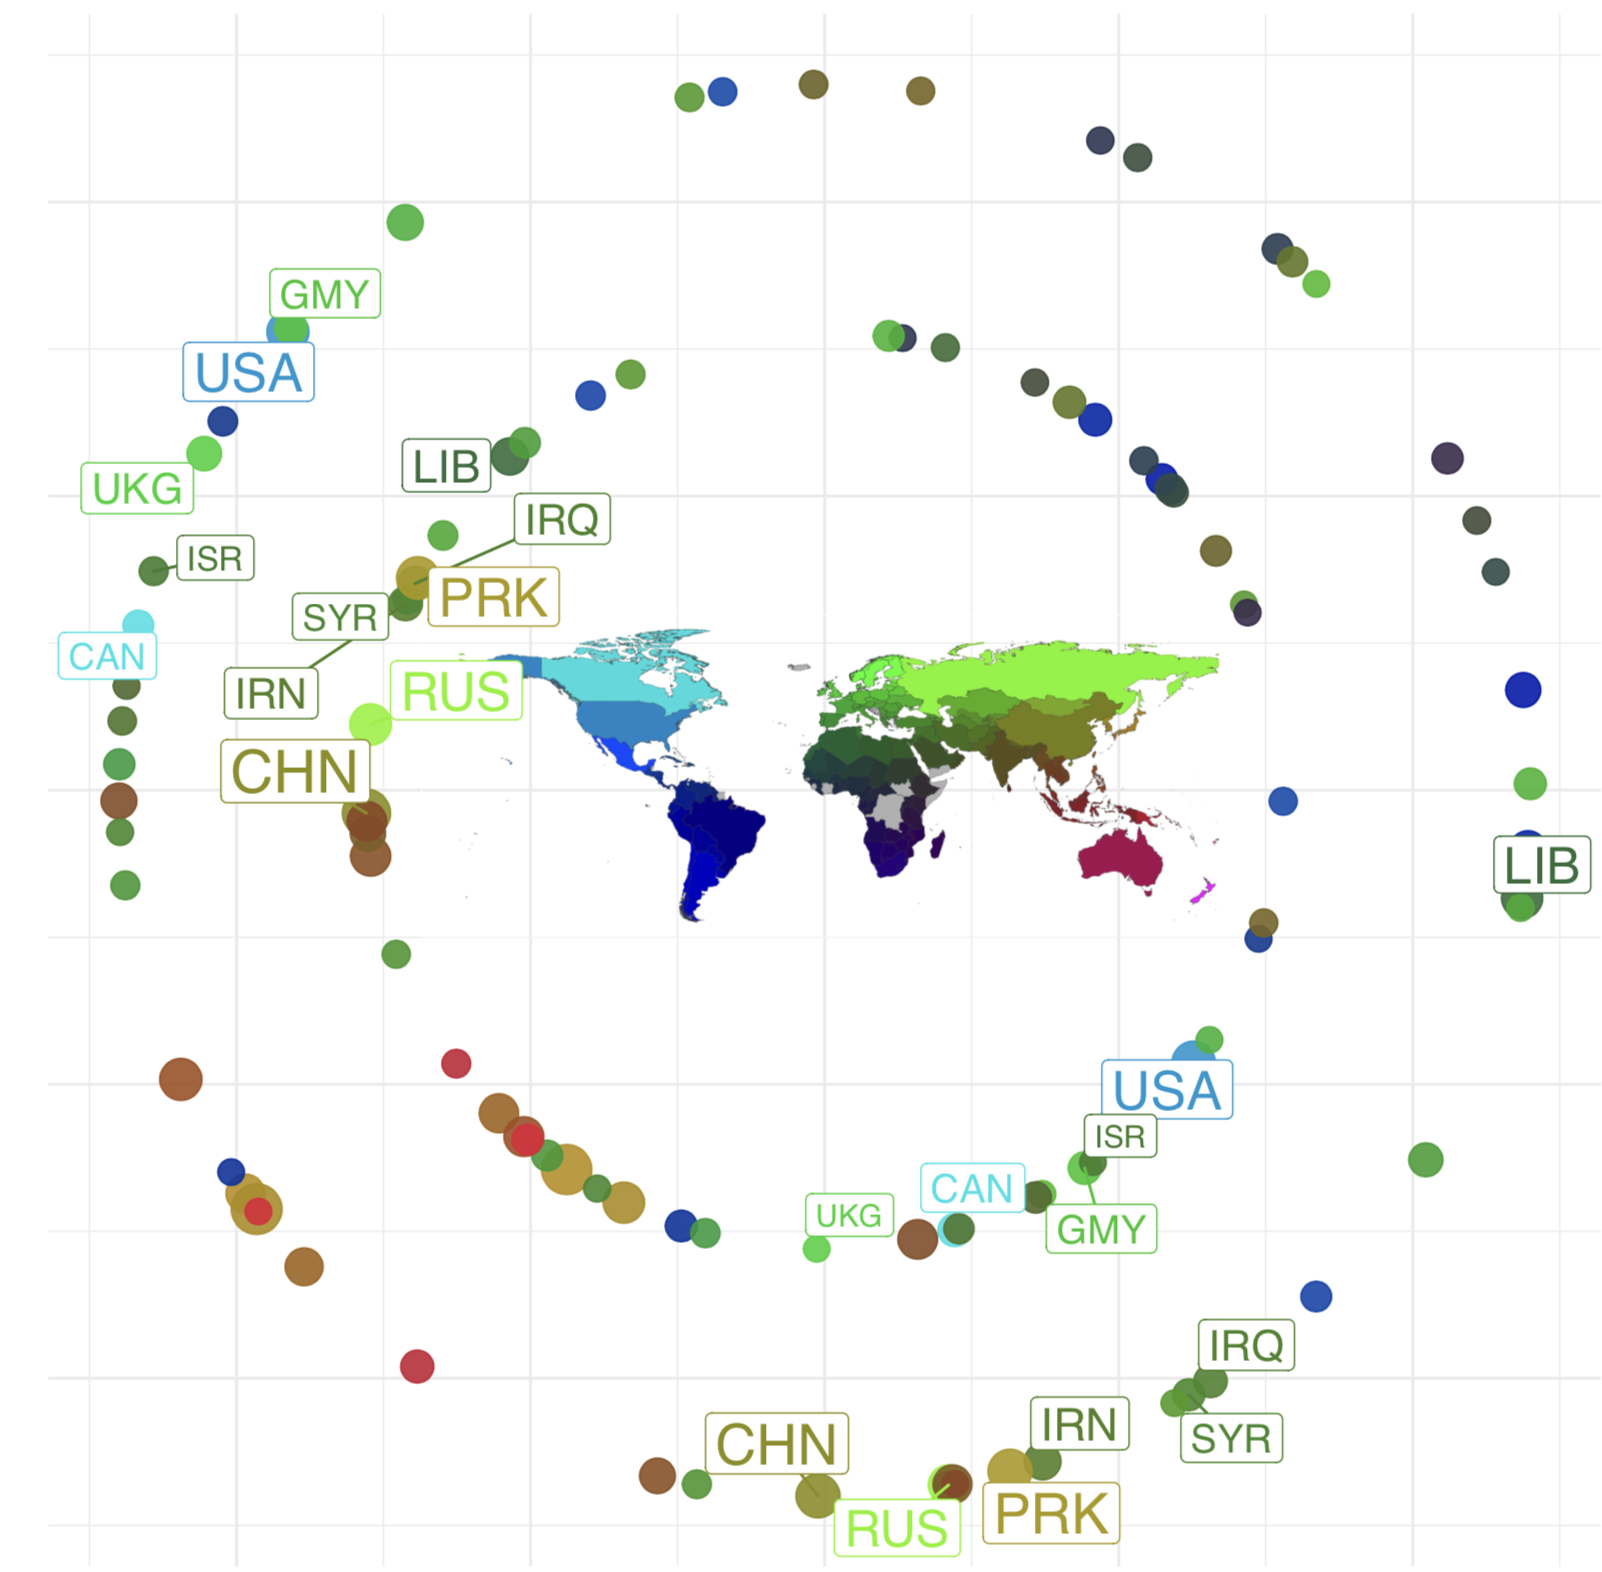
\includegraphics[width=\textwidth]{graphics/weeks_circPlot.png}
	\caption{ Visualization of multiplicative effects for Weeks (2012). Each circle designates a country and the color corresponds to the legend at the center of the visualization. Countries that cluster together in the outer ring are those that were found by the model to have similar sending patterns, meaning that they tend to send conflict to similar sets of countries. The inner ring clusters countries by the similarity of who they receive conflict from. 
	}
	\label{fig:weekscirc}
\end{figure}
\FloatBarrier

To visualize the multiplicative effects, we develop the circular diagram shown in Figure~\ref{fig:weekscirc}. The nodes throughout the diagram represent countries and they are colored according to their geographic position -- a legend is provided in the center. The outer ring visualizes higher order dependence patterns that countries have in terms of their sending relationships -- country positions here are estimated in the $\mathbf{u}_{i}$ random effects described in Equation~\ref{eqn:ame}. Countries that are more proximate to each other in this outer ring are more likely to send or initiate conflictual events with similar targets. The inner ring, based on estimates of $\mathbf{v}_{i}$, is constructed such that countries more proximate to each other are more likely to receive conflict from the same countries. Last, the distance between countries in the inner and outer rings proportionately reflects who a country is more likely to be in conflict with. 

Interestingly, when examining Figure~\ref{fig:weekscirc} we quickly are able to reveal a number of clusters. For example, in the top left corner we see the US, UK, Germany, Canada, and Israel. These states cluster together in the outer ring of this visualization because they tend to send conflicts to similar targets. Conversely, in the bottom right of the outer ring, we see a cluster of authoritarian countries: Iraq, Russia, Syria, North Korea, and China. We see similar clusters develop in the inner ring, specifically, we again see the US, UK, Germany, Canada, and Israel clustering together indicating that they are more likely to receive conflict from the same countries. Additionally, we again see authoritarian regimes like North Korea, Iraq, and Syria clustering. Further, the cluster of democratic and authoritarian countries are facing each other in the inner and outer rings, indicating that they are more likely to be in conflict with one another. 

Most important, in evaluating this visualization we are actually able to see some of Weeks' logic play out in terms of how states behave in the conflict system. Specifically, Iraq, Syria, Libya, and North Korea all fell under Weeks' ``boss" category, and each of these states tends to cluster together in the inner and outer rings. This indicates that even though we do not find support for Weeks' assertion that certain authoritarian regime types are more likely to initiate conflict, we do find that these regimes are more likely to behave similarly in terms of who they are more likely to target and receive conflict from. 

\subsection{Gibler (2017)}

The last re-estimation we conduct with the AME model involves a study by \citet{gibler:2017}. Gibler argues that the long-standing relationship between the relative parity of capabilities and initiation of militarized interstate disputes (MIDs) is almost completely mediated by the initial conditions for the members of the dyad when they joined the international system as sovereign members. This finding calls into question many IR theories about the role of balance in terms of generating international conflict \citep{organski:1958}.

To test this hypothesis, Gibler employs an undirected dyadic design and estimates his model using a GLM with dyad clustered standard errors.\footnote{Full tabular results are shown in the appendix, we focus on model 6 from Table 6 (2017, 34).} With this design, Gibler finds support for his primary variable, parity of the members of a dyad at the year in which they entered the international system. However, when we reestimate using AME, this measure becomes too imprecisely measured for us to draw any inferences about its effect on the initiation of MIDs. Not only is our estimate of the effect of Gibler's parity variable small, but it has a very large relative standard error---over a magnitude larger than the parameter itself. 

In the two previous replications, we showed how to parse apart underlying structure using the SRM and LFM portions of the AME framework. Here we turn our focus to parameter interpretation in a substantive context. Specifically, even when the GLM and AME frameworks produce results that may seem to be in accordance with one another, the substantive interpretations of the effects of covariates can differ notably as the AME model uses a set of random effects to account for unobserved factors. To do this, we focus on the effect of rivalry in the onset of a MID. Both the GLM and AME estimations find that rivalry has a positive effect on MID initiation, but the expected effects the two models provide are quite stark.

To clarify the difference, we turn to a simulation based approach. We employ mean or modal values for all independent variables, except we change the rivalry variable to indicate that there was a rivalry when the actual data suggest there is none. This provides us with two scenarios, one in which rivalry is set to one and the other zero, while in both scenarios all other parameters are set to their measure of central tendency. The expected values of this scenario are essentially a first difference plot comparing results with the model when estimated in two different ways: the GLM estimation and our AME approach.  

\begin{figure}
	\caption{Marginal effects of a change in the Rivalry variable for both the AME and the Gibler estimation.  \label{fig:gibmargeff}}
	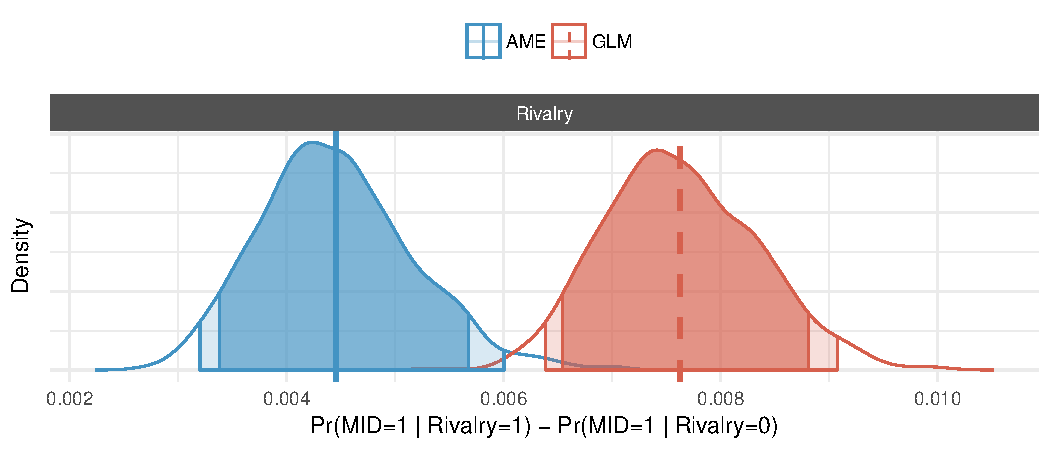
\includegraphics[width=\textwidth]{graphics/gibler_margeff.pdf}
 	\label{fig:gibmargeff}
 \end{figure}

As Figure~\ref{fig:gibmargeff} illustrates, the substantive results differ notably. First, the expected value of the dependent variable---the probability of the onset of a militarized interstate dispute, is considerably lower when taking interdependencies into account with the AME model.  These are rare events, so the probabilities are low, but the difference is a factor of almost 2. Thus, you get quite substantially different expected values from these two models.  

\subsection{Lessons Learned}

First, utilizing the AME framework enables scholars to better model the underlying structure that dyadic data often comes with. In each of the replications, the predictive performance in an out-of-sample context of the AME framework is notably superior. Specifically, not only does AME perform better at correctly identifying cases in which the dependent variable takes a value of $0$ (via the ROC curves), but it also dominates at correctly identifying occurrences of the dependent variable in the data (seen via the PR curves). 

Second, in both the simulation section and these replications we have shown that results can change notably when interdependencies are not taken into account. Not only are coefficients biased in the GLM approaches to the analysis of dyadic data, but they are often imprecisely measured, with poorly calibrated standard errors.  This means that significance testing (for better or worse) is compromised when network effects are ignored.

Third, even when the results from the AME estimation conform with those found in an OLS or logistic regression, new insights can emerge from the structure that the random effects of the AME framework uncover. In particular, there is actual information about the dependencies so that clusters can be identified, and this information can also be used to generate new hypotheses. This kind of information is absent in standard approaches and adds to our ability to explain specific as well as general results.

Fourth, it is evident that the actual results---not the estimated coefficients and their covariances---which are generated by the models differ greatly in expectations.  This implies that policy experimentations with the models, as well as scenario-based simulations and forecasting of GLM models are likely to often give misleading results compared to the AME approach.
